\documentclass[pdftex]{article}
% \documentclass[prl,showpacs,amsmath,amssymb]{revtex4} % PRL

% margins of 1 inch:
\setlength{\topmargin}{-.5in}
\setlength{\textheight}{9in}
\setlength{\oddsidemargin}{0in}
\setlength{\textwidth}{6.5in}

\usepackage[pdftex]{hyperref} % hyperlink equation and bibliographic citations
\usepackage[dvips]{graphicx,color}
\usepackage{amsmath} % advanced math
\usepackage{verbatim} % multi-line comments
\usepackage{natbib} % bibilography
\usepackage{mciteplus} % collapse multiple citations in bibilography

% from http://www.flakery.org/search/show/569

\newcommand{\infint}{\ensuremath{\int_{-\infty}^{\infty}}}

\newcommand{\ie}{\textit{i.e.}\ }
\newcommand{\eg}{\textit{e.g.}\ }

\newcommand{\eqn}[1]{Eq.\ (\ref{#1})}

\newcommand{\pfrac}[2]{\ensuremath{\frac{\partial #1}{\partial #2}}}

\begin{document}

\title{Network Model}

\author{Ben Payne$^{1}$\footnote{Electronic address: bpayne@lps.umd.edu}
{\it $^{1}$Department of Fun, University Name \& Town, city, State Zip}}

\date{\today}

% \begin{abstract}
% Model random networks
% \end{abstract}

%\maketitle % declares end of title page

\tableofcontents

%\newpage

\section{Introduction}

There are two methods to model a network:
\begin{itemize}
 \item create a database of port connections
 \item create autonomous routers which direct packets to other components
\end{itemize}
For this model I will be using a database of connections.

\subsection{problem}

All possible compute bottlenecks:
\begin{itemize}
 \item CPU clock rate
 \item memory (L1, L2, RAM, disk) access latency
 \item memory (L1, L2, RAM, disk) access bandwidth
 \item network bandwidth
 \item network latency
\end{itemize}

We want an efficient and reasonable all-to-all network. 

An optimal all-to-all design would have each compute node with $N-1$ ports and no routers (0 hops).
\begin{figure}[h!]
\begin{center}
(a)\ \includegraphics[scale=0.2]{pictures/N2_n1_M0_mNA}\ \ \ 
(b)\includegraphics[scale=0.2]{pictures/N3_n1_M0_mNA}\ \ \ 
(c)\ \includegraphics[scale=0.2]{pictures/N4_n1_M0_mNA}\ \ \ 
(d)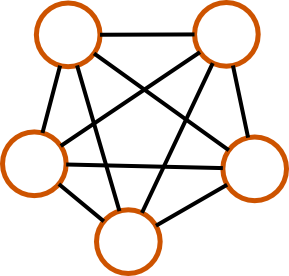
\includegraphics[scale=0.2]{pictures/N5_n1_M0_mNA}\\*
\caption{increasing the number of nodes. Doesn't scale well due to limited number of ports on each compute node ($n<N$).}
\end{center}
\end{figure}
For $N>1000$ this simplisitic approach is not feasiable. Thus we introduce routers.
\begin{figure}[h!]
\begin{center}
(a)\includegraphics[scale=0.2]{pictures/N4_n1_M1_m4}\ \ \ 
(b)\includegraphics[scale=0.2]{pictures/N6_n1_M2_m4}\\*
\caption{adding routers. Doesn't scale well due to limited number of ports per router ($m<N$). Also, conjestion (a,b) and bisection bandwidth (a) are poor.}
\end{center}
\end{figure}

To reduce conjestion and increase bisection bandwidth, add more routers. Also increase the number of ports per compute node. Then the optimization problem becomse non-trivial.

\subsection{objectives}

If I can show a given topology is better than some other, that is useful.

If I can show how one router versus another (differentiated by number of ports) affects performance, that is useful.

Note: although this model is useful for all-to-all communication measurement, there are not inherent constraints as far as applying this same model to other interests. You can use whatever fitness function you can define.

\subsection{Does Topology matter? A toy model example}

Suppose now we have $N=5$ compute nodes with 1 port each. Then the optimal network design (fewest hops) is to have a 5 port router:
\begin{figure}[h!]
\begin{center}
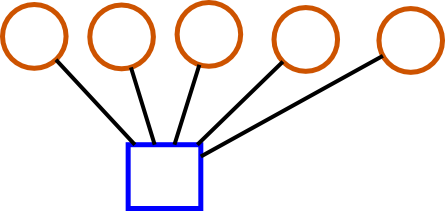
\includegraphics[scale=0.2]{pictures/N5_n1_M1_m5.png}\\*
\caption{Here number of hops is 1 for each compute node, with 10 pairs (=5*4/2).}
\end{center}
\end{figure}

The other extreme would be to use five of these same routers with only one compute node per router:
\begin{figure}[h!]
\begin{center}
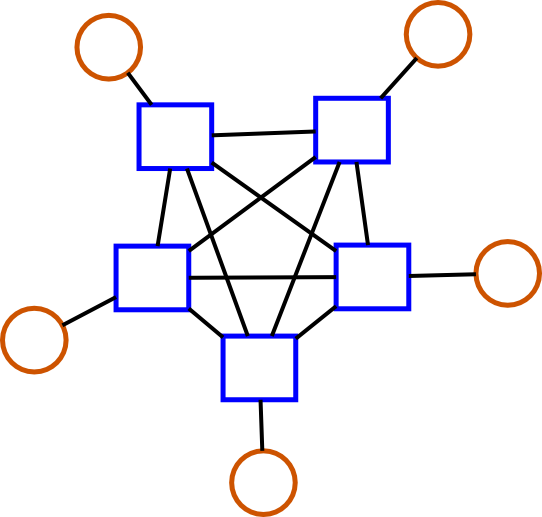
\includegraphics[scale=0.2]{pictures/N5_n1_M5_m5.png}\\*
\caption{Here number of hops is 2 for each compute node.}
\end{center}
\end{figure}
Clearly we are spending too much money on routers for the same number of compute nodes. However, this increased hop count (2) also lowers conjestion.

As a compromise, we can use two routers and increase the number of compute nodes:

\begin{figure}[h!]
\begin{center}
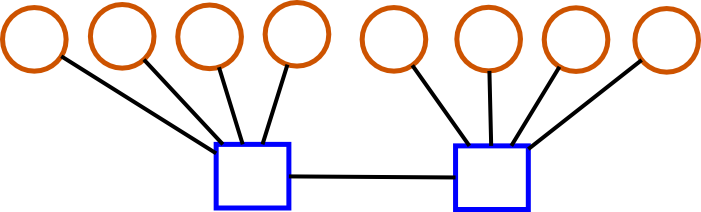
\includegraphics[scale=0.2]{pictures/N8_n1_M2_m5.png}\\*
\caption{8 nodes and 2 routers: 12 pairs with 1 hop, 16 pairs with 2 hops.}
\end{center}
\end{figure}

\begin{figure}[h!]
\begin{center}
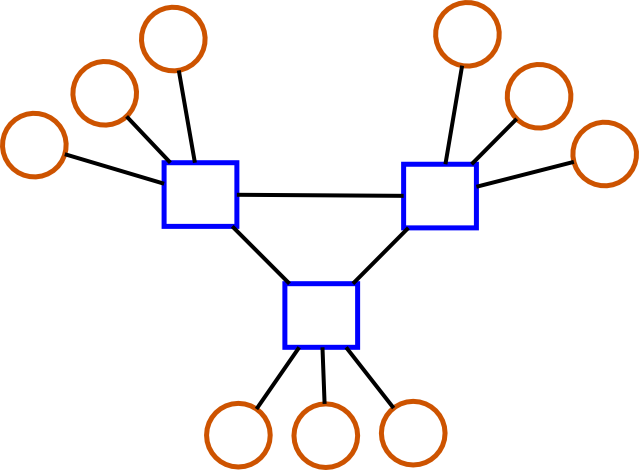
\includegraphics[scale=0.2]{pictures/N9_n1_M4_m5.png}\\*
\caption{1 or 2 hops, 9 nodes and 3 routers.}
\end{center}
\end{figure}
Notice a few constraints were followed:
\begin{itemize}
 \item each router has same number of ports
 \item each compute node has one port
 \item each router is fully occupied
 \item each node can reach every other node
 \item each router has at least one computer connected to it
\end{itemize}

The number of permutations increases when we have more than 9 compute nodes and only 5 ports. Even worse, consider when there are multiple ports per computer (but much less than the number of computers).

The parameter space includes
\begin{itemize}
 \item number of computers
 \item number of ports per computer
 \item number of routers
 \item number of ports per router
\end{itemize}
Metrics:
\begin{itemize}
 \item hop count for each pair
 \item bisection bandwidth
\end{itemize}


\subsection{Permutations}

The number of unique pairs on a network swith $N$ computers is $N(N-1)/2$. 

When $N=4$ then there are 6 pairs. $N=100$ is 4950 pairs. $N=10,000$ is 49,995,000 pairs.

\section{standard networks}

See \href{http://www.cs.nmsu.edu/~pfeiffer/classes/573/notes/topology.html}{http://www.cs.nmsu.edu/~pfeiffer/classes/573/notes/topology.html}

\subsection{Mesh}
Mesh (and the related torus) can be of $n$ dimensions, commonly $n=$2, 3, 6. Useful for physical sciences due to local communication (nearest neighbors).
\begin{comment}
##Command to produce the output: "neato -Tpng thisfile.gv > thisfile.png"
##Command to produce the output: "circo -Tpng thisfile.gv > thisfile.png"
graph G {
node [shape=box,color=red,style=bold];  c0;
node [shape=box,color=red,style=bold];  c1;
node [shape=box,color=red,style=bold];  c2;
node [shape=box,color=red,style=bold];  c3;
node [shape=box,color=red,style=bold];  c4;
node [shape=box,color=red,style=bold];  c5;
node [shape=box,color=red,style=bold];  c6;
node [shape=box,color=red,style=bold];  c7;
node [shape=box,color=red,style=bold];  c8;
node [shape=circle,fixedsize=true,width=0.9,color=blue,style=bold];  s0;
node [shape=circle,fixedsize=true,width=0.9,color=blue,style=bold];  s1;
node [shape=circle,fixedsize=true,width=0.9,color=blue,style=bold];  s2;
node [shape=circle,fixedsize=true,width=0.9,color=blue,style=bold];  s3;
node [shape=circle,fixedsize=true,width=0.9,color=blue,style=bold];  s4;
node [shape=circle,fixedsize=true,width=0.9,color=blue,style=bold];  s5;
node [shape=circle,fixedsize=true,width=0.9,color=blue,style=bold];  s6;
node [shape=circle,fixedsize=true,width=0.9,color=blue,style=bold];  s7;
node [shape=circle,fixedsize=true,width=0.9,color=blue,style=bold];  s8;
     s0--c0;
     s1--c1;
     s2--c2;
     s3--c3;
     s4--c4;
     s5--c5;
     s6--c6;
     s7--c7;
     s8--c8;
     s0--s1; 
     s0--s3;
     s1--s2;
     s1--s4;
     s2--s5;
     s3--s4;
     s3--s6;
     s4--s7;
     s4--s5;
     s5--s8;
     s6--s7;
     s7--s8;
     overlap=false
     label="3x3 mesh\nlayed out by Graphviz"
     fontsize=12;
}
\end{comment}
Mesh networks are well-characterized. ``Meshes have O(n) cost, O(sqrt(n)) bisection bandwidth, O(n) aggregate bandwidth, and O(sqrt(n)) latency.''

\begin{figure}[h!]
\begin{center}
 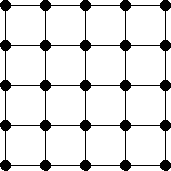
\includegraphics[scale=.5]{pictures/mesh}
\end{center}
\end{figure}



\subsection{Hypercube}

``the latency is is O(log N). There are N processors, each with log2N interfaces, so the cost is O(N log N). and all the processors can use their links simultaneously, so our aggregate bandwidth is O(N). The bisection bandwidth is O(log N).''

\subsection{Omega}

``scales as $n \log n$.''

\subsection{Fat Tree}

\href{http://en.wikipedia.org/wiki/Fat_tree}{http://en.wikipedia.org/wiki/Fat\_tree}

\subsection{Flattened Butterfly}

\subsection{Dragonfly}

\href{http://research.google.com/pubs/pub34926.html}{http://research.google.com/pubs/pub34926.html}

Fractal

\subsection{Clos Network}

\href{http://en.wikipedia.org/wiki/Clos_network}{http://en.wikipedia.org/wiki/Clos\_network}

\subsection{randomly-connected networks}

For networks supporting physical models (i.e., mesh), it makes sense to think about dimension, perimeter/surface area, area/volume. This may not apply to scale-free topologies. 

If the topology turns out to be scale free, then we wouldn't need to model 1E6 endpoints (that is desirable).

\section{more than one port per endpoint}

If each computer endpoint has only one network connection, and all routers have the same configuration of router and computer connections, then we can model a router-only network. 

This might simplify the analysis, but here we model more complicated networks. Routers which don't necessarily have the same configuration, compute nodes with more than one port. Then it is necessary to include both ``router'' and ``compute'' type nodes.

\section{random network creation}

For a given \{(number of computers), (number of ports per computer), (number of ports per router)\}, should random computers be plugged into random port routers, or should random routers be connected first?

\ \\
``connections'' database methods:
\begin{itemize}
 \item each router is an sub-array of the connections array. The elements of each sub-array denote which computer the router is plugged into. 
 \item connections pairs: computer--router and router-router. The connections array has sub-arrays of size 2 for each edge of the graph (nodes are either computers or routers).
 \begin{itemize}
  \item unordered pairs of positive (router) and negative (computer) integer indices
 \end{itemize}

\end{itemize}
Features needed:
 \begin{itemize}
  \item support routers having arbitrary port count (not all routers must have same number of ports)
  \item no router connects to itself
 \end{itemize}


\ \\
Whether local symmetry (same number of computers plugged into each router) is a hinderance, benefit, or irrelevant is not clear to me.

Random connections lead to unexpected paths. This could be good, bad, or inconsequential.

\section{route enumeration}

\begin{enumerate}
 \item For each computer, see what other computers are available on the same router (1 hop)
 \item For each computer, see what other computers are two routers away (2 hops)
 \item ...
\end{enumerate}
When a router has had all of its computers touched for a given iteration, then we should mark that router as ``touched'' (doesn't need to be queried again for current iteration). That is, mark a router to indicate ``all locally-attached computers have number of hops known.'' This should reduce search time.

\section{Maximum and Minimum number routers needed}
How many routers ($M$) are needed when each router has $m$ ports? (Assume $m<(N-1)$.)

Variables: 
\begin{itemize}
 \item $n$ = number ports per compute node
 \item $N$ = number of compute nodes
\item $m$ = number of ports per router
 \item $M$ = number of routers
\end{itemize}
Observe that we have already made the simplifying assumption of identical compute nodes and identical routers.

\subsection{one port per compute node}
For $N$ compute nodes, how many routers $M$ are needed when each router has $m$ ports? We assume there are more compute nodes than ports on one router ($m<(N-1)$). We must obey the constraints (every compute node must be able to reach every other compute node -- ``fully connected network''), (all router ports are used), (all compute node ports are used).

\textbf{Solution 1}: to get an all-to-all network, each node should connect to a tree with $(N-1)$ endpoints (bisection bandwidth is thus maximized). To acheive this, start with one compute node and a router with $m$ ports (for this example let $m=5$). At this tree level ($k=1$) we have $m=5$, $M'=1$, and $N-1=4$. ($M'$ refers to the number of routers for this one compute node).

\begin{figure}[h!]
\begin{center}
\includegraphics[scale=0.3]{pictures/N5_n1_M1_m5_tree}
\label{fig:tree_k1}
 \caption{$m=5$, $M'=1$, $N-1=4$ (tree level $k=1$). }
\end{center}
\end{figure}

\begin{figure}[h!]
\begin{center}
\includegraphics[scale=0.3]{pictures/N17_n1_M5_m5_tree}
\label{fig:tree_k2}
 \caption{$m=5$, $M'=1+4$, $N-1=4*4$ (tree level $k=2$). }
\end{center}
\end{figure}


\begin{figure}[h!]
\begin{center}
\includegraphics[scale=0.3]{pictures/N65_n1_M21_m5_tree}
\label{fig:tree_k3}
 \caption{$m=5$, $M'=1+4+4^2$, $N-1=4^3$ (tree level $k=3$). }
\end{center}
\end{figure}

Generalizing, the number of compute nodes the one we are dealing with can connect to is
\begin{equation}
 N-1=(m-1)^k
 \label{eq:Nminus1k}
\end{equation}
and the number routers this one compute node needs to create $N-1$ endpoints is
\begin{equation}
 M'=\sum_{a=1}^{k} (m-1)^{(a-1)}
\end{equation}
Since there are a total of $N$ compute nodes, the total number of routers $M$ needed is
\begin{equation}
\boxed{
 M_{max}=N\sum_{a=1}^{k} (m-1)^{(a-1)}
 }
\end{equation}
This is the maximum number of routers needed.

We can solve for $k$ from Eq.~\ref{eq:Nminus1k}
\begin{equation}
 \log(N-1)=k\log(m-1)
\end{equation}
\begin{equation}
 k=\frac{\log(N-1)}{\log(m-1)}
 \label{eq:k_n1}
\end{equation}
valid values: $m>2$ and $N>2$.

For Matlab/Octave,
\begin{verbatim}
 a=1:ceil(log(N-1)/log(m-1)); M_max=N*sum((m-1).^(a-1))
\end{verbatim}
Note: use of ``ceil'' gives worse case scenario in which there are empty router ports. This equation is accurate when Eq.~\ref{eq:k_n1} is an integer (then ``ceil'' is not used).

\textbf{Solution 2}: the minimum number of routers needed can be found by daisy-chaining routers together. We can enumerate this by seeing how many compute nodes can be attached to 1 router, then 2 routers, and so on. 

\begin{figure}[h!]
\begin{center}
\includegraphics[scale=0.3]{pictures/N5_n1_M1_m5}
\label{fig:neq15}
 \caption{$m=5$, $M=1$, $N=5$}
\end{center}
\end{figure}

\begin{figure}[h!]
\begin{center}
\includegraphics[scale=0.3]{pictures/N8_n1_M2_m5}
\label{fig:neq18}
 \caption{$m=5$, $M=2$, $N=4+4=8$}
\end{center}
\end{figure}

\begin{figure}[h!]
\begin{center}
\includegraphics[scale=0.3]{pictures/N11_n1_M3_m5}
\label{fig:neq111}
 \caption{$m=5$, $M=3$, $N=4+3+4$}
\end{center}
\end{figure}

\begin{figure}[h!]
\begin{center}
\includegraphics[scale=0.3]{pictures/N14_n1_M4_m5}
\label{fig:neq114}
 \caption{$m=5$, $M=4$, $N=4+3+3+4$}
\end{center}
\end{figure}

Thus, for $M>1$, 
\begin{equation}
 N=(m-1)+(M-2)(m-2)+(m-1)=2(m-1)+(M-2)(m-2)
\end{equation}
This solution has a high hop count and low bisection bandwidth of 1.

Solving for $M$,
\begin{equation}
\boxed{
M_{min}= \frac{N-2(m-1)}{m-2}+2
}
\label{eq:maximum_neq1}
\end{equation}
where $m>2$ and $N>2(m-1)$.

For Matlab/Octave,
\begin{verbatim}
M_min=(N-(2*(m-1)))/(m-2)+2 
\end{verbatim}


\ \\
As an example, when $N=1000$ and $m=24$, the maximum number of routers is 553,000 (solution 1) and the minimum is 46 (solution 2).

\subsection{more than one port per compute node}
What is the maximum router count when there are two ports per compute node ($n=2$)? 

\textbf{Solution 1} (maximum number of routers): Start with one compute node and a router with $m$ ports (for this example let $m=5$). At this tree level ($k=1$) we have $m=5$, $M'=2$, and $N-1=2*4=8$. ($M'$ refers to the number of routers for this one compute node).


\begin{figure}[h!]
\begin{center}
\includegraphics[scale=0.3]{pictures/N9_n2_M2_m5_tree}
\label{fig:ngt1k1}
 \caption{$m=5$, $M'=2$, $N-1=2*4$ (tree level $k=1$). }
\end{center}
\end{figure}

\begin{figure}[h!]
\begin{center}
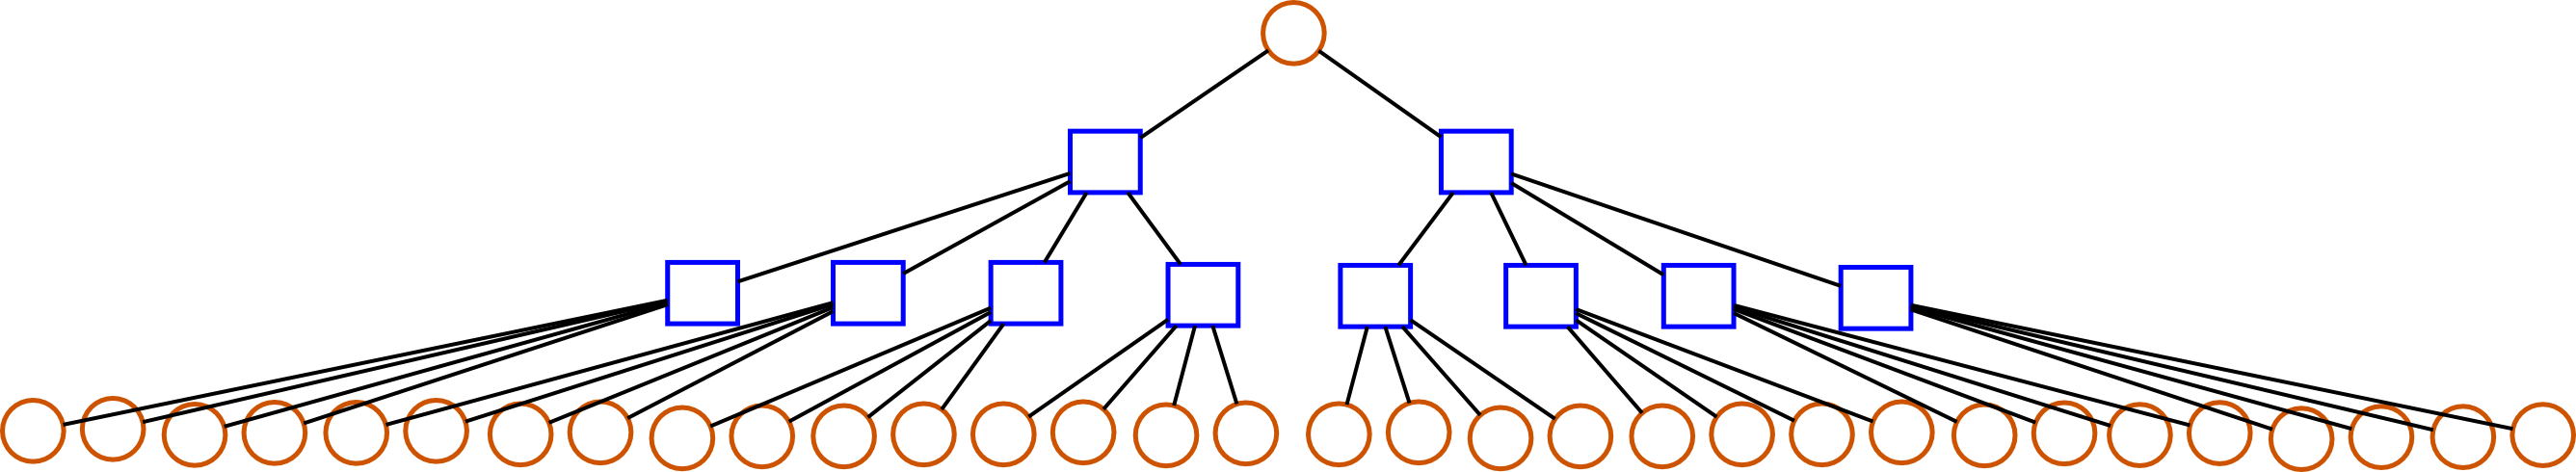
\includegraphics[scale=0.3]{pictures/N33_n2_M10_m5_tree}
\label{fig:ngt1k2}
 \caption{$m=5$, $M'=2+2*4$, $N-1=2*4*4$ (tree level $k=2$). }
\end{center}
\end{figure}

% \begin{figure}[h!]
% \begin{center}
% \includegraphics[scale=0.3]{pictures/}
% \label{fig:ngt1k2}
%  \caption{$m=5$, $M'=2+2*4$, $N-1=2*4*4$ (tree level $k=2$). }
% \end{center}
% \end{figure}


% \begin{figure}[h!]
% \begin{center}
% \includegraphics[scale=0.3]{pictures/}
% \label{fig:ngt1k3}
%  \caption{$m=5$, $M'=2+2*4+4^2$, $N-1=2*4^3$ (tree level $k=3$). }
% \end{center}
% \end{figure}

Generalizing, the number of nodes this one can connect to is
\begin{equation}
 N=n(m-1)^k
 \label{eq:Nminus1kngt1}
\end{equation}
and the number of routers for this one compute node is
\begin{equation}
 M'=n\sum_{a=1}^{k} (m-1)^{(a-1)}
\end{equation}
As before, the total number of routers needed is $M=N M'$,
\begin{equation}
\boxed{
 M_{max}=N n\sum_{a=1}^{k} (m-1)^{(a-1)}
 }
 \label{eq:maximum_ngt1}
\end{equation}
and we can solve Eq.~\ref{eq:Nminus1kngt1} to find $k$
\begin{equation}
 \log(N-1)=\log(n) + k\log(m-1)
\end{equation}
\begin{equation}
 k=\frac{\log((N-1)/n)}{\log(m-1)}
 \label{eq:k_many_n}
\end{equation}

For Matlab/Octave,
\begin{verbatim}
a=1:ceil(log((N-1)/n)/log(m-1)); M_max=N*n*sum((m-1).^(a-1))
\end{verbatim}
Note: use of ``ceil'' gives worse case scenario in which there are empty router ports. This equation is accurate when Eq.~\ref{eq:k_many_n} is an integer (then ``ceil'' is not used).

The maximum number of routers as given by Eq.~\ref{eq:maximum_ngt1} is expected to be less than the value from Eq.~\ref{eq:maximum_neq1} since there are more ports supplied at the compute node.

\textbf{Solution 2} (minimum number of routers): Again we will start with $n=2$ and find how many compute nodes are supported with 1 router, then 2 routers, and so on. Here we will assume $m=4$. We cannot use one router for two compute nodes because it violates our earlier assumption that no compute node should connect to the same router twice.

With two routers, we can connect 4 compute nodes.

\begin{figure}[h!]
\begin{center}
\includegraphics[scale=0.3]{pictures/N4_n2_M2_m4}
\label{fig:ngt14}
 \caption{$m=4$, $M=2$, $N=4$.}
\end{center}
\end{figure}


\begin{figure}[h!]
\begin{center}
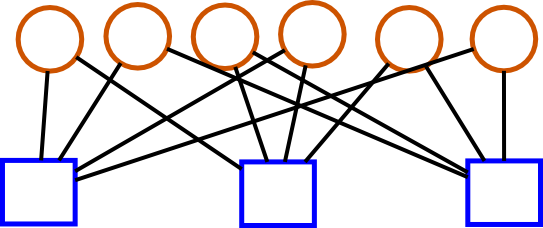
\includegraphics[scale=0.3]{pictures/N6_n2_M3_m4}
\label{fig:ngt16}
 \caption{$m=4$, $M=3$, $N=6$.}
\end{center}
\end{figure}

Clearly this becomes a mess to enumerate systematically. The important point is that the minimum number of routers is higher when $n>1$. This is to be expected since there are more connections per compute node. Compare Fig.~\ref{fig:ngt14},~\ref{fig:ngt16} and Fig.~\ref{fig:fewer_routers_M1},~\ref{fig:fewer_routers_M2}

\begin{figure}[h!]
\begin{center}
\includegraphics[scale=0.3]{pictures/N4_n1_M1_m4}
\label{fig:fewer_routers_M1}
 \caption{$m=4$, $M=1$, $N=4$.}
\end{center}
\end{figure}

\begin{figure}[h!]
\begin{center}
\includegraphics[scale=0.3]{pictures/N6_n1_M2_m4}
\label{fig:fewer_routers_M2}
 \caption{$m=4$, $M=2$, $N=6$.}
\end{center}
\end{figure}



\ \\
As an example using the same parameters as before, when $N=1000$ and $m=24$, the maximum number of routers is now 72,000 (solution 1) and the minimum is greater than the minimum found when $n=1$. The maximum was expected to decrease (compared to the maximum for $n=1$) since there are more ports at the compute node.

\ \\
As a check, the difference between the maximum and minimum number of routers should go to zero as $n$ approaches $N-1$. 

\begin{figure}[h!]
\begin{center}
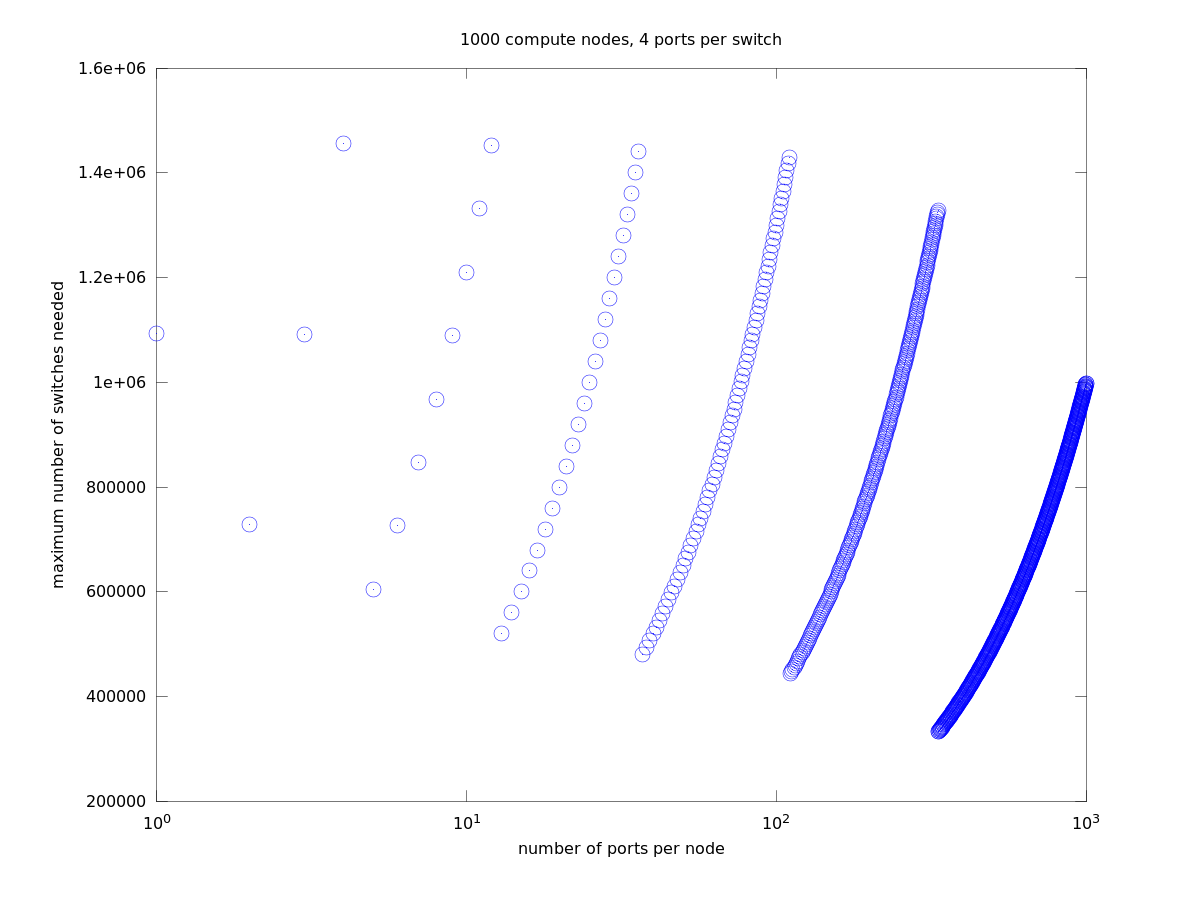
\includegraphics[scale=.3]{pictures/maximum_number_of_routers_needed_versus_compute_node_port_count_for_1000_compute_nodes_and_4_ports_per_router_semilogx}
\label{fig:max}
 \caption{$m=4$, $M=3$, $N=6$.}
\end{center}
\end{figure}
\begin{verbatim}
 N=1000; m=4; 
 for n=1:(N-1),
   a=1:ceil(log((N-1)./n)./log(m-1));
   M_max(n)=N*n.*sum((m-1).^(a-1));
 end
 n=1:(N-1);
 plot(n,M_max)
 figure; plot(1:N-2,M_max,"o","markersize",15)
 xlabel("number of ports per node"); ylabel("maximum number of routers needed"); title("1000 compute nodes, 4 ports per router")
 print -dpng maximum_number_of_routers_needed_versus_compute_node_port_count_for_1000_compute_nodes_and_4_ports_per_router.png
 print -deps maximum_number_of_routers_needed_versus_compute_node_port_count_for_1000_compute_nodes_and_4_ports_per_router.eps
 figure; semilogx(1:N-2,M_max,"o","markersize",15)
 xlabel("number of ports per node"); ylabel("maximum number of routers needed"); title("1000 compute nodes, 4 ports per router")
 print -dpng maximum_number_of_routers_needed_versus_compute_node_port_count_for_1000_compute_nodes_and_4_ports_per_router_semilogx.png
 print -deps maximum_number_of_routers_needed_versus_compute_node_port_count_for_1000_compute_nodes_and_4_ports_per_router_semilogx.eps
 figure; loglog(1:N-2,M_max,"o","markersize",15)
 xlabel("number of ports per node"); ylabel("maximum number of routers needed"); title("1000 compute nodes, 4 ports per router")
 print -dpng maximum_number_of_routers_needed_versus_compute_node_port_count_for_1000_compute_nodes_and_4_ports_per_router_loglog.png
 print -deps maximum_number_of_routers_needed_versus_compute_node_port_count_for_1000_compute_nodes_and_4_ports_per_router_loglog.eps
\end{verbatim}
 
\section{network alterations}

\subsection{swap computer connections}

\begin{enumerate}
 \item pick random pair from connections database {[}cA, s1]
 \item pick random pair from connections database {[}cB, s2]
 \item check that (cA != cB) and (s1 != s2)
 \item check that the suggested rearrange ``{[}cA, s1] and {[}cB, s2] transform to {[}cA, s2] and {[}cB, s1] in connections database'' doesn't create an invalid network (i.e., more than one of the compute ports plugged into the same router)
 \item rearrange: {[}cA, s1] and {[}cB, s2] transform to {[}cA, s2] and {[}cB, s1] in connections database
\end{enumerate}

Note: we actually could let the evolution include ``invalid'' networks (i.e., multiple computer ports plugged into same router). However, this would probably result in a longer evolution (if the optimal network doesn't include this redundancy).

\subsection{swap router connections}

\begin{enumerate}
 \item pick random pair from connections database {[}s1, X]
 \item pick random pair from connections database {[}s2, Y]
 \item check that (X != Y) and (s1 != s2)
 \item check that the suggested rearrange ``{[}s1, X] and {[}s2, Y] transform to {[}s2, X] and {[}s1, Y] in connections database'' doesn't create an invalid network (i.e., more than one of the compute ports plugged into the same router)
 \item rearrange: {[}s1, X] and {[}s2, Y] transform to {[}s1, Y] and {[}s2, X] in connections database
\end{enumerate}

It appears that ``swap router connections'' and ``swap computer connections'' have sufficient overlap that they can be merged to one routine.

\subsection{swapping sets of connections on routers}

\begin{enumerate}
 \item pick random pair from connections database {[}s1, X1]
 \item pick random pair from connections database with same router, {[}s1, X2]
 \item pick random pair from connections database {[}s2, Y1]
 \item pick random pair from connections database with same router, {[}s1, Y2]
 \item check that (s1 != s2) and  (X1 != Y1) and (X1 != Y2) and (X2 != Y1)\\
 Note that we don't have to check either (X1 != X2) or (Y1 != Y2) as this is done when the initial valid network is created
 \item check that the suggested rearrange doesn't create an invalid network 
 \item rearrange: {[}s1, X1], {[}s1, X2], {[}s2, Y1], {[}s2, Y2] transform to {[}s1, Y1], {[}s1, Y2], {[}s2, X1], {[}s2, X2] in connections database
\end{enumerate}

Q: is swapping multiple ports between two routers distinct from performing the same number of swaps on individual port pairs on routers?\\
For example,\\
``{[}s1, X1], {[}s1, X2], {[}s2, Y1], {[}s2, Y2] transform to {[}s1, Y1], {[}s1, Y2], {[}s2, X1], {[}s2, X2]'' is equivalent to\\
``{[}s1, X1], {[}s2, Y1] transforms to {[}s1, Y1], {[}s2, X1]\\
and\\
{[}s1, X2], {[}s2, Y2] transforms to {[}s1, Y2], {[}s2, X2]''

\section{Fitness functions}

\subsection{bisection bandwidth}
Page 52 of the thesis ``A complexity theory for VLSI'' by C. Thompson (1980) defines bisection bandwidth for communication graphs as half the compute nodes being separated.

How to measure bisection bandwidth: chose a random set of half the compute nodes. Determine how many cuts need to be made to separate the two halves. There are many possible combinations of routers, and which nodes are in which half also matters.

Question posted to \href{https://groups.google.com/d/topic/networkx-discuss/hv_SzY-uaTw/discussion}{Networkx Google Group}

Question: how to halve the compute nodes?\\

Simplification: consolidate compute nodes which are on the same router. This only applies to compute nodes with one port.

Idea: use strong repulsion between the compute nodes?

Does recording the paths between compute nodes help?

\subsubsection{number of bisections}
How many times does the bisection need to be measured?

To answer this, we need to know how many unique permutations there are of the network. Suppose there are $N$ computers and $M$ routers. Then the number of halves of computers is $N(N-1)(N-2)\cdots(N/2)$:
\begin{equation}
 \prod_{x=0}^{N/2}(N-x)
\end{equation}
Similarly, the number of (unequal) router partitions is $M!$. Thus the number of unique network partitions, $U$, is
\begin{equation}
 U = M! \prod_{x=0}^{N/2}(N-x)
\end{equation}
If we want to find the minimum bisection, then an (orderly) exhaustive search is necessary. Instead, do a random search (random swaps of edges) and have some confidence of having found the minimum.

Given $U$ items, how many picks $p$ are needed to get a specific item with a certain confidence level $q$. Constraints: (1) the search $p$ doesn't stop when the item is found, (2) picks are made with replacement -- there are always $U$ items.

As an example, suppose $U=2$. Then $p=1$ gives $q=50\%$. The confidence increases when $p$ increases, but it never reaches 100\%. For $p=2$, the outcomes in which we find the specific item are
 (($p_1$ and $p_2$) or ($p_1$ and $!p_2$) or ($!p_1$ and $p_2$)). Thus $p=2$ yeilds $q=.5*.5+.5*.5+.5*.5=$75\%. An easier way of expressing this is to ask the opposite: which outcomes are not going to yield the specific item? When we don't pick it in all tries: ($!p_1$ and $!p_2$). Then we care about 1-(.5*.5)=75\%.

One more pick, $p=3$. The cases in which we find a specific item are the same as not finding it after 3 tries: $1-(!p_1$ and $!p_2$ and $!p_3)=1-(.5*.5*.5)=$87.5\%. 

Since $p_i=1/U$, then $!p_i=1-(1/U)$.
 
Once we can find the confidence based on $p$ picks, we can invert the relation and calculate the number of picks needed to have a certain confidence level. Given $p$ picks of $U$ items, the confidence $C$ that the specific item was picked at least once is
\begin{equation}
 C = 1 - \left(1-\frac{1}{U}\right)^p
\end{equation}
Invert this to find $p(C,U)$
\begin{equation}
  \left(1-\frac{1}{U}\right)^p = 1-C
\end{equation}
\begin{equation}
 p = \frac{\log(1-c)}{\log(1-(1/U))}
\end{equation}
As an example, suppose we want 90\% confidence ($C=0.9$) and there are 100 items to pick from ($U=100$). Then
\begin{equation}
 p = \lceil\frac{\log(1-.9)}{\log(1-(1/100))}\rceil = 230
\end{equation}
We would need 230 picks.

\subsection{hop count}

\href{http://en.wikipedia.org/wiki/Shortest_path_problem}{http://en.wikipedia.org/wiki/Shortest\_path\_problem}

Problem: Given connections
\begin{equation}
 [[-1,4],[-2,4],[-2,5],[-3,5],[3,5],[1,3],[1,2],[2,4]]
\end{equation}
See Fig.~\ref{fig:wrong_hop_count}.
\begin{figure}
\begin{center}
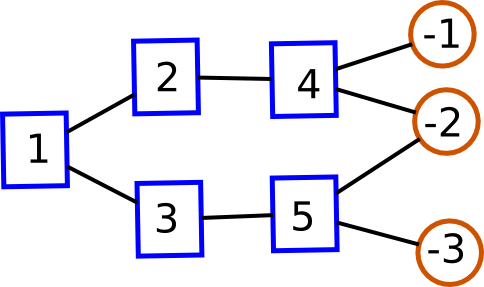
\includegraphics[scale=.3]{pictures/N3_n2_M5_m2}
\label{fig:wrong_hop_count}
 \caption{$m=1,2$, $M=5$, $N=3$. The hop count between -1 and -3 is 6, not 4.}
\end{center}
\end{figure}
Routes between compute nodes can only use positive nodes.

Objective: seek the shortest path between two negative nodes which contain no negative nodes.

Method: for $A<0$ and $B<0$, create a new graph with nodes $A$, $B$, and all positive nodes. Then find the shortest path between $A$ and $B$. Repeat for all compute node pairs.

\subsection{single-source shortest path}

\href{http://en.wikipedia.org/wiki/Dijkstra\%27s_algorithm}{http://en.wikipedia.org/wiki/Dijkstra\%27s\_algorithm}

\subsubsection{All pairs shortest Path}

\begin{itemize}
 \item \href{http://en.wikipedia.org/wiki/Floyd\%E2\%80\%93Warshall_algorithm}{http://en.wikipedia.org/wiki/Floyd\%E2\%80\%93Warshall\_algorithm}
 \item \href{http://www.cs.rochester.edu/u/nelson/courses/csc_173/graphs/apsp.html}{http://www.cs.rochester.edu/u/nelson/courses/csc\_173/graphs/apsp.html}
 \item \href{http://stackoverflow.com/questions/5249857/all-pairs-all-paths-on-a-graph}{http://stackoverflow.com/questions/5249857/all-pairs-all-paths-on-a-graph}
\end{itemize}
Might be able to get away with finding average hop count and maximum hop count if (1) that is all we care about and (2) there's a faster algorithm for those counts.
%  \begin{itemize}
%   \item average hop count
%   \item maximum hop count
%  \end{itemize}


\subsection{Multi-objective optimization}
 
When a fitness function has multiple components, i.e.,
\begin{equation}
 f=a(\textrm{cost})+b(\textrm{latency})+c(\textrm{bisection\ bandwidth})
\end{equation}
Then how do you chose values for $a$, $b$, and $c$? The outcome of the evolution is expected to be sensitive to changes in each.
 
\section{problems}
 
\section{future task list}

Once the hop counter is implemented, it would be useful to validate metrics against analytic values for mesh, torus, fat tree topologies.


\end{document}
